%%%%%%%%%%%%%%%%%%%%%%%%%%%%%%%
%%Derived from "Metropolis" (beamerthememetropolis)
%
% May need to run 
% 1) LaTex -> PDF
% 2) LaTex -> DVI -> PDF
% 3) LaTex -> DVI -> PS -> PDF
% 4) XeTex -> PDF
%
%%%%%%%%%%%%%%%%%%%%%%%%%%%%%%%%%%%%%%



%%%%%%%%%%%%%%%%%%%
% BEAMER CHOICES
%%%%%%%%%%%%%%%%%%%

\documentclass{beamer}
\mode<presentation>{\usetheme{metropolis}}


%%%%%%%%%%%
% PACKAGES
%%%%%%%%%%%

\usepackage[english]{babel}
\usepackage[latin1]{inputenc}
\usepackage{times}
\usepackage[T1]{fontenc}

\usepackage{comment}
\usepackage{amsmath}
\usepackage{amsthm}                           % Required for theorem environments
\usepackage{bm}                               % Required for bold math symbols (used in the footer of the slides)
\usepackage{graphicx}                         % Required for including images in figures
\usepackage{booktabs}                         % Required for horizontal rules in tables
\usepackage{multicol}                         % Required for creating multiple columns in slides
\setlength{\columnsep}{0.1mm}
\usepackage{lastpage}                         % For printing the total number of pages at the bottom of each slide
\usepackage{microtype}                        % Better typography
\usepackage{tocstyle}                         % Required for customizing the table of contents
\usepackage{caption}
\captionsetup{labelformat=empty,labelsep=none}
\usepackage{mathtools}
\usepackage{subcaption}
\usepackage{nicefrac}
\usepackage{csquotes}

\usepackage{enumitem}	                        %spread enumeration over multiple slides
\usepackage{pdfpages}
\usepackage{tikz}  
\usepackage[absolute, overlay]{textpos}      %position textblocks (absolute) on the page
\setlength{\TPHorizModule}{\textwidth}
\setlength{\TPVertModule}{\textwidth}


\usepackage{appendixnumberbeamer}
\usepackage{booktabs}
\usepackage{xspace}
 \newcommand{\themename}{\textbf{\textsc{metropolis}}\xspace}



%%%%%%%%%%%%%%%%%%%%%%%%%%%%%%%
% TITLE PAGE AND BEAMER OPTIONS
%%%%%%%%%%%%%%%%%%%%%%%%%%%%%%%%

\title{The Logic of Science}
\subtitle{(or why common sense makes sense) }
\date{\today}
\author{Bruce D. Marron}
%\institute{Dynamic Ecosystems and Landscapes Lab; North Carolina State University}
\titlegraphic{
\begin{tikzpicture}[overlay]
  \node[anchor=south west] at (0,-8.5) {
\includegraphics[scale= 0.2]{graphics/DEAL_lab.png}};
  \node[anchor=south west] at (6,-8.5) {
\includegraphics[scale= 0.05]{graphics/ncstate.jpg}};  
 \end{tikzpicture}
 }

%---------------OPTIONALS-------------------------------------------------------
% (optional, use only with lots of authors)
%\author[Author, Another] {F.~Author\inst{1} \and S.~Another\inst{2}}

% \institute[Universities of Somewhere and Elsewhere] 
% {  \inst{1}%
%  Department of Computer Science\\
%  University of Somewhere
%  \and
%  \inst{2}%
%  Department of Theoretical Philosophy\\
%  University of Elsewhere
%  }

% (optional, should be abbreviation of conference name)
%\date[CFP 2003] {Conference on Fabulous Presentations, 2003}

% This is only inserted into the PDF information catalog. Can be left out. 
%\subject{Theoretical Computer Science}


% the table of contents pops up at the beginning of each subsection
%\AtBeginSubsection[]                                     
% {
%  \begin{frame}<beamer>{Outline}
%    \tableofcontents[currentsection,currentsubsection]
%  \end{frame}
% }


% uncover everything in a step-wise fashion
%\beamerdefaultoverlayspecification{<+->}              
%-----------------------------------------------------------------------------------------------------


%%%%%%%%%%%%%%%%%%%%%%%%%
% SPECIALTY NEW COMMANDS
%%%%%%%%%%%%%%%%%%%%%%%%%%
 
% Arrow over vector
\newcommand{\amsvect}{%
  \mathpalette {\overarrow@\vectfill@}}
\def\vectfill@{\arrowfill@\relbar\relbar{\raisebox{-3.81pt}[\p@][\p@]{$\mathord\mathchar"017E$}}}


% Nice-looking fractions
\newcommand\ddfrac[2]{\frac{\displaystyle #1}{\displaystyle #2}}





%#############
%  SLIDES
%#############


\begin{document}

%---------------------------------
\begin{frame}
  \titlepage
\end{frame}

%-----------------------------------
\begin{comment}
\begin{frame}{The Overview}
  \tableofcontents
  % You might wish to add the option [pausesections]
\end{frame}
\end{comment}

%----------------------------------

\section{The Answer}

%-----------------------------------
\begin{frame}

\begin{align*}
 P(H_f | D ) &= P(H_f) \ddfrac{(P(D | H_f)}{P(D)} \\
&= \ddfrac{P_fL_f}{P_fL_f + P_pL_p + \sum{P_iL_i}} \\
& \sim 0.47
\end{align*} 

\end{frame}

%----------------------------------

\section{The Wonderment}

%---------------------------------------------------
\begin{frame}{I wonder ....}

\begin{tikzpicture}[overlay]
  \node[anchor=south west] at (5.5,-4.5) {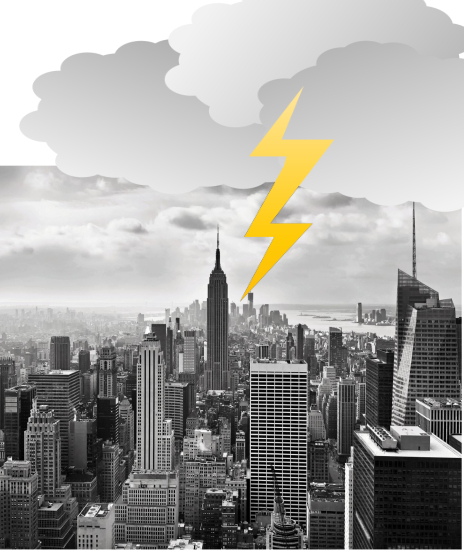
\includegraphics[scale=.45]{graphics/lightning1.jpeg}};  
 \end{tikzpicture}
 
\begin{textblock}{1}(.05,.21)
  \normalsize {Can cityscapes \textbf{influence} weather?}
\end{textblock}

\end{frame}

%--------------------------------------------------------------
\begin{frame} {I wonder ....}
\begin{tikzpicture}[overlay]
  \node[anchor=south west] at (5.5,-4.5) {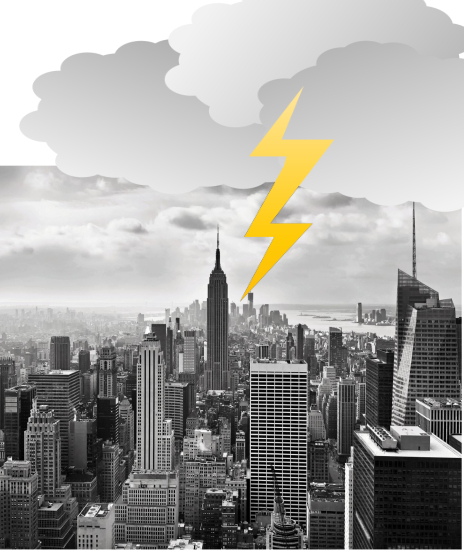
\includegraphics[scale=.45]{graphics/lightning1.jpeg}};  
 \end{tikzpicture}
 
\begin{textblock}{1}(.05,.21)
  \normalsize {Can cityscapes \textbf{influence} weather?}
\end{textblock}
 

\begin{textblock}{1}(.125,.26)
  \normalsize {Can cityscapes \textbf{generate} weather?}
\end{textblock}
\end{frame}

%---------------------------------------------------------------
\begin{frame} {I wonder ....}
\begin{tikzpicture}[overlay]
  \node[anchor=south west] at (5.5,-4.5) {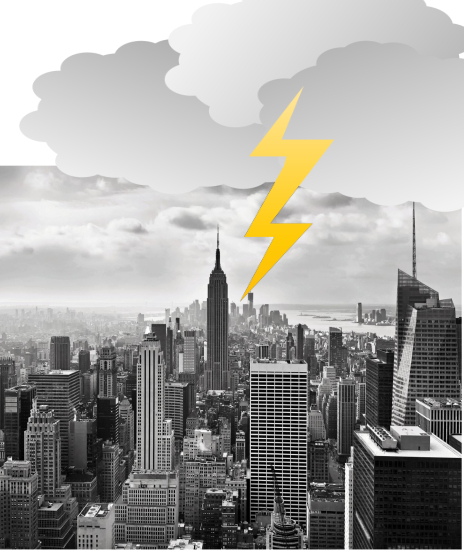
\includegraphics[scale=.45]{graphics/lightning1.jpeg}};  
 \end{tikzpicture}
 
\begin{textblock}{1}(.05,.21)
  \normalsize {Can cityscapes \textbf{influence} weather?}
\end{textblock}
 

\begin{textblock}{1}(.125,.26)
  \normalsize {Can cityscapes \textbf{generate} weather?}
\end{textblock}
 
  
\begin{textblock}{1}(.225,.31)
  \normalsize {Can cityscapes \textbf{cause} thunderstorms?}
\end{textblock}
\end{frame}


\section{The Master}

%-------------------------------------------------------------------
\begin{frame}{The logic of science: From reality to models and back again}

\begin{tikzpicture}[overlay]
  \node[anchor=south west] at (6.25,-3.5) {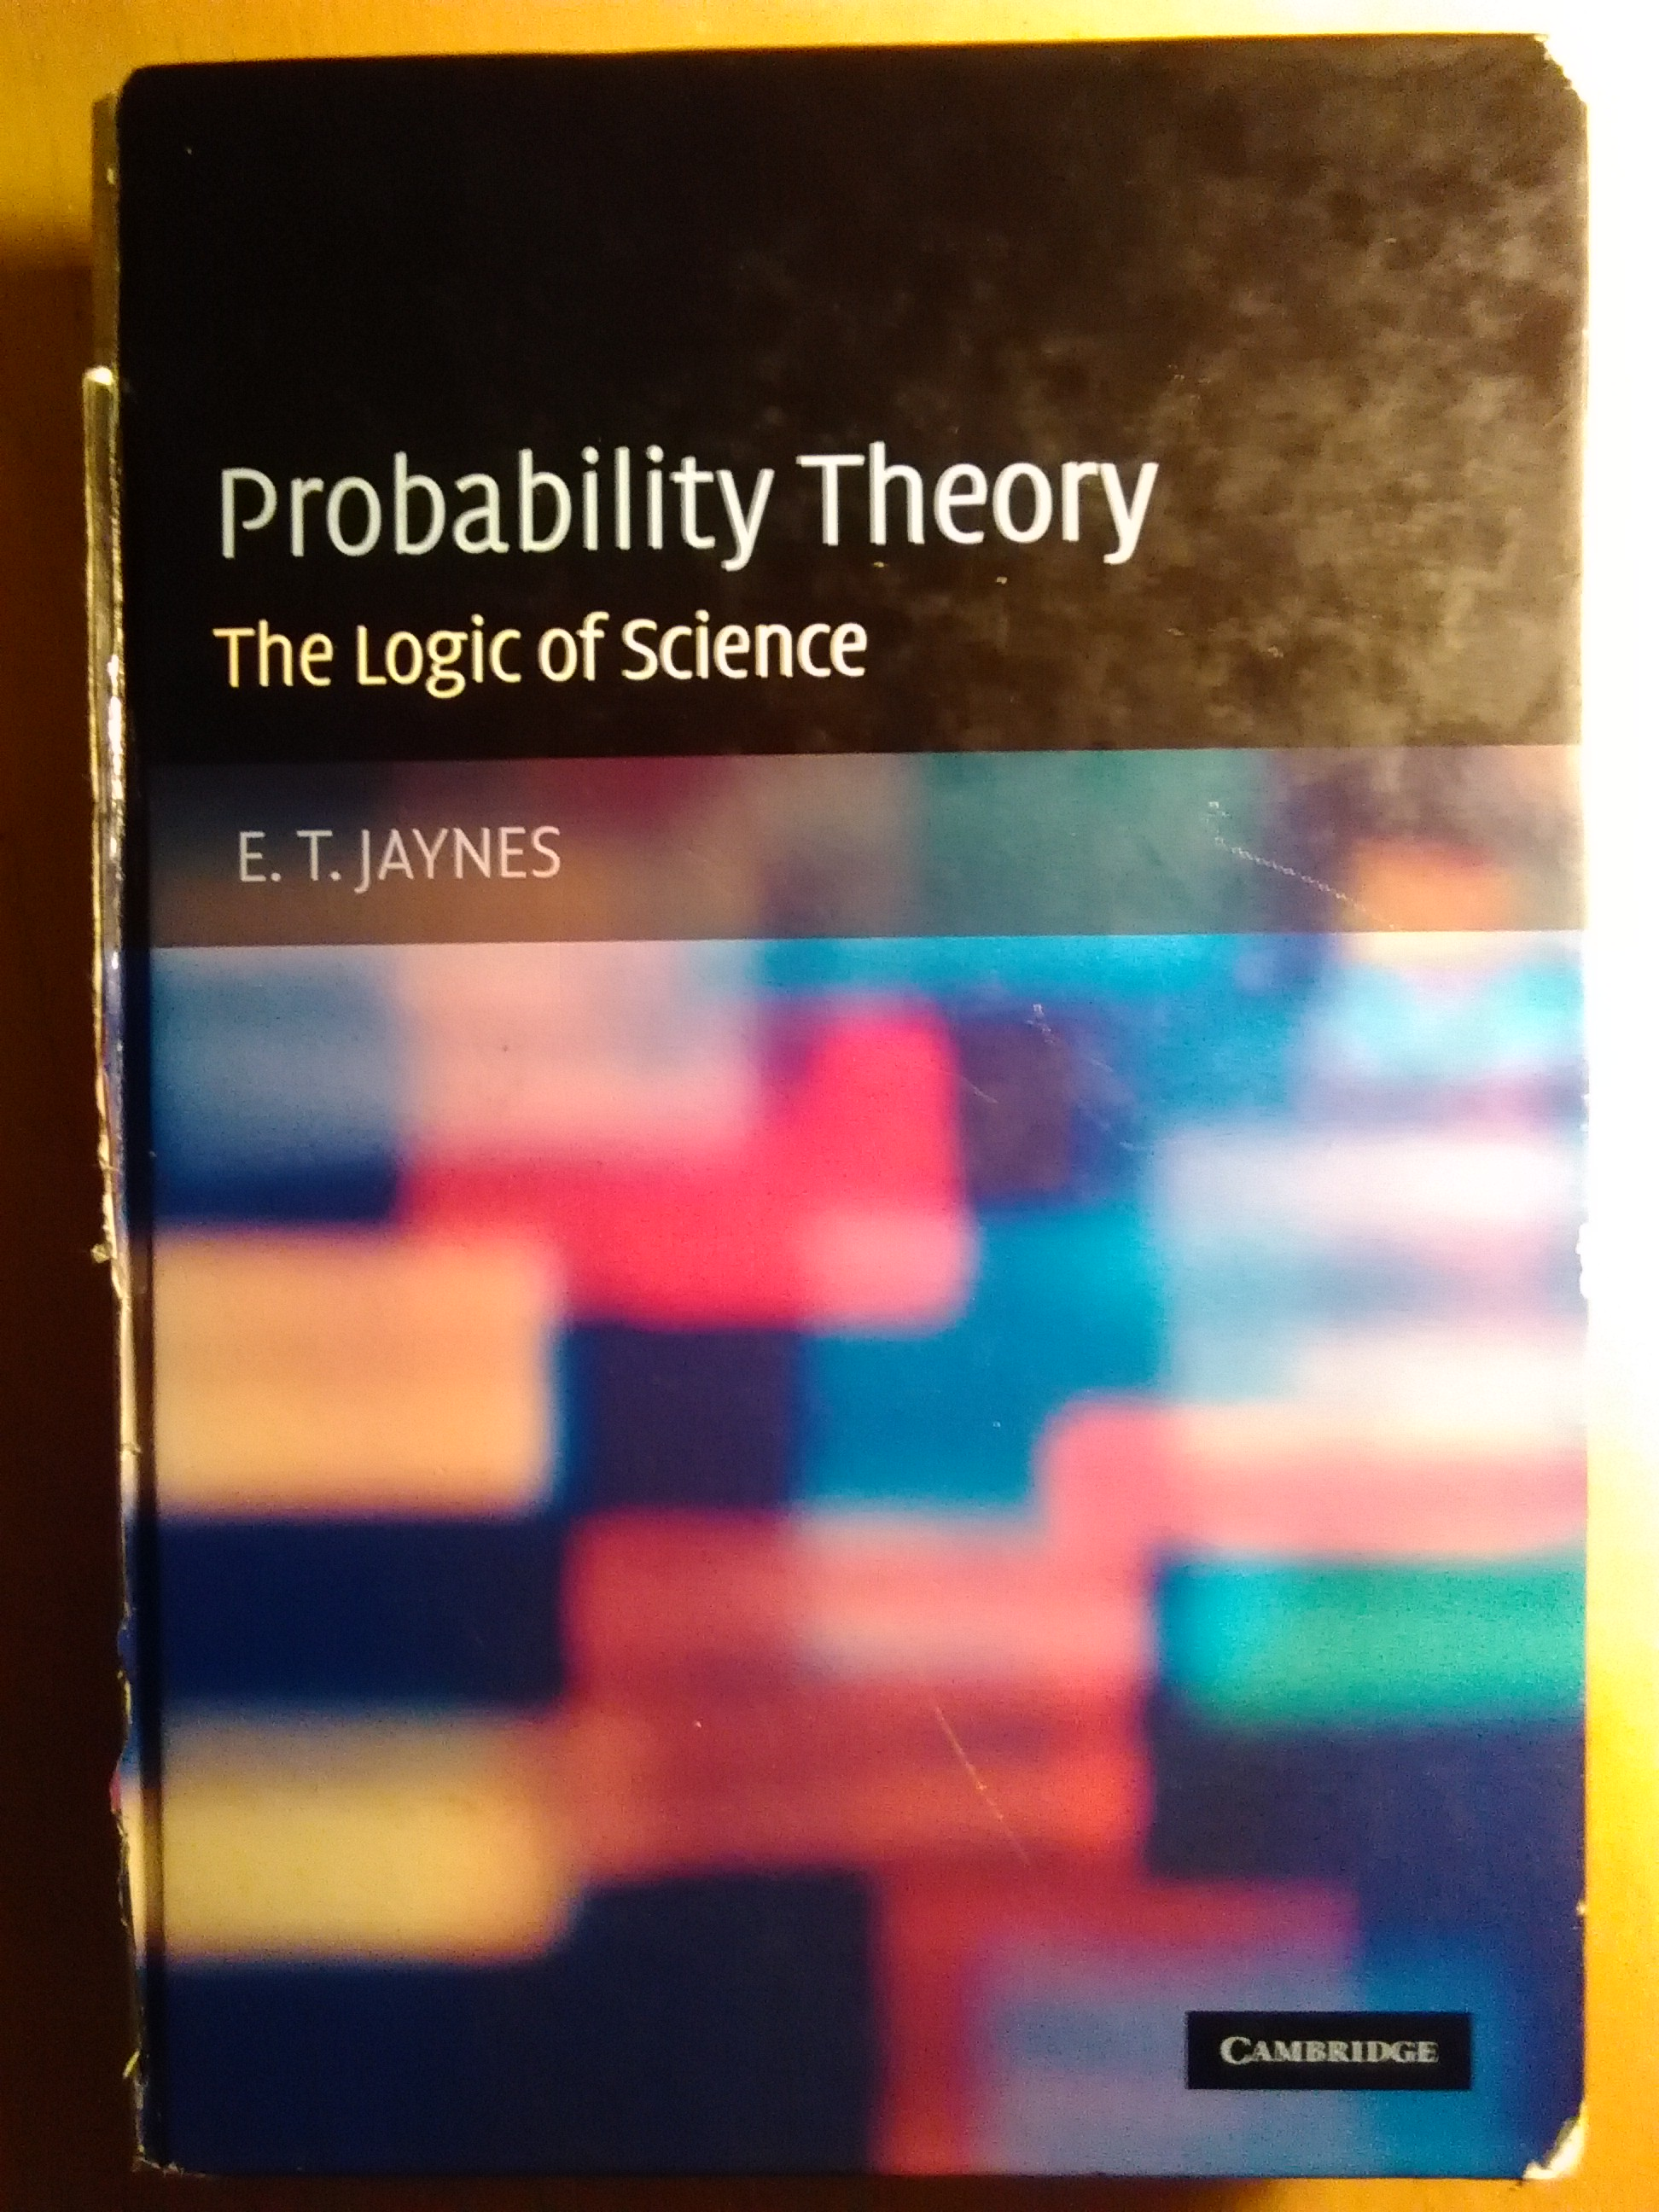
\includegraphics[scale=.070]{graphics/Jaynes.jpg}};  
 \end{tikzpicture}
 
\begin{textblock}{1}(.045,.40)
  \small {"In virtually all real problems of scientific \\
  inference...the problem facing the scientist \\
  is of the inverse type: Given the data D, \\
  what is the probability that some \\
  hypothesis H is true?"}
\end{textblock}

\begin{textblock}{1}(.2,.70)
  \tiny {--- E.T. Jaynes (2003, p.85)}
\end{textblock}

\end{frame}


\section{The Science}

%----------------------------------------------------------------
\begin{frame}

\begin{tikzpicture}[overlay]
  \node[anchor=south west] at (1,-4) {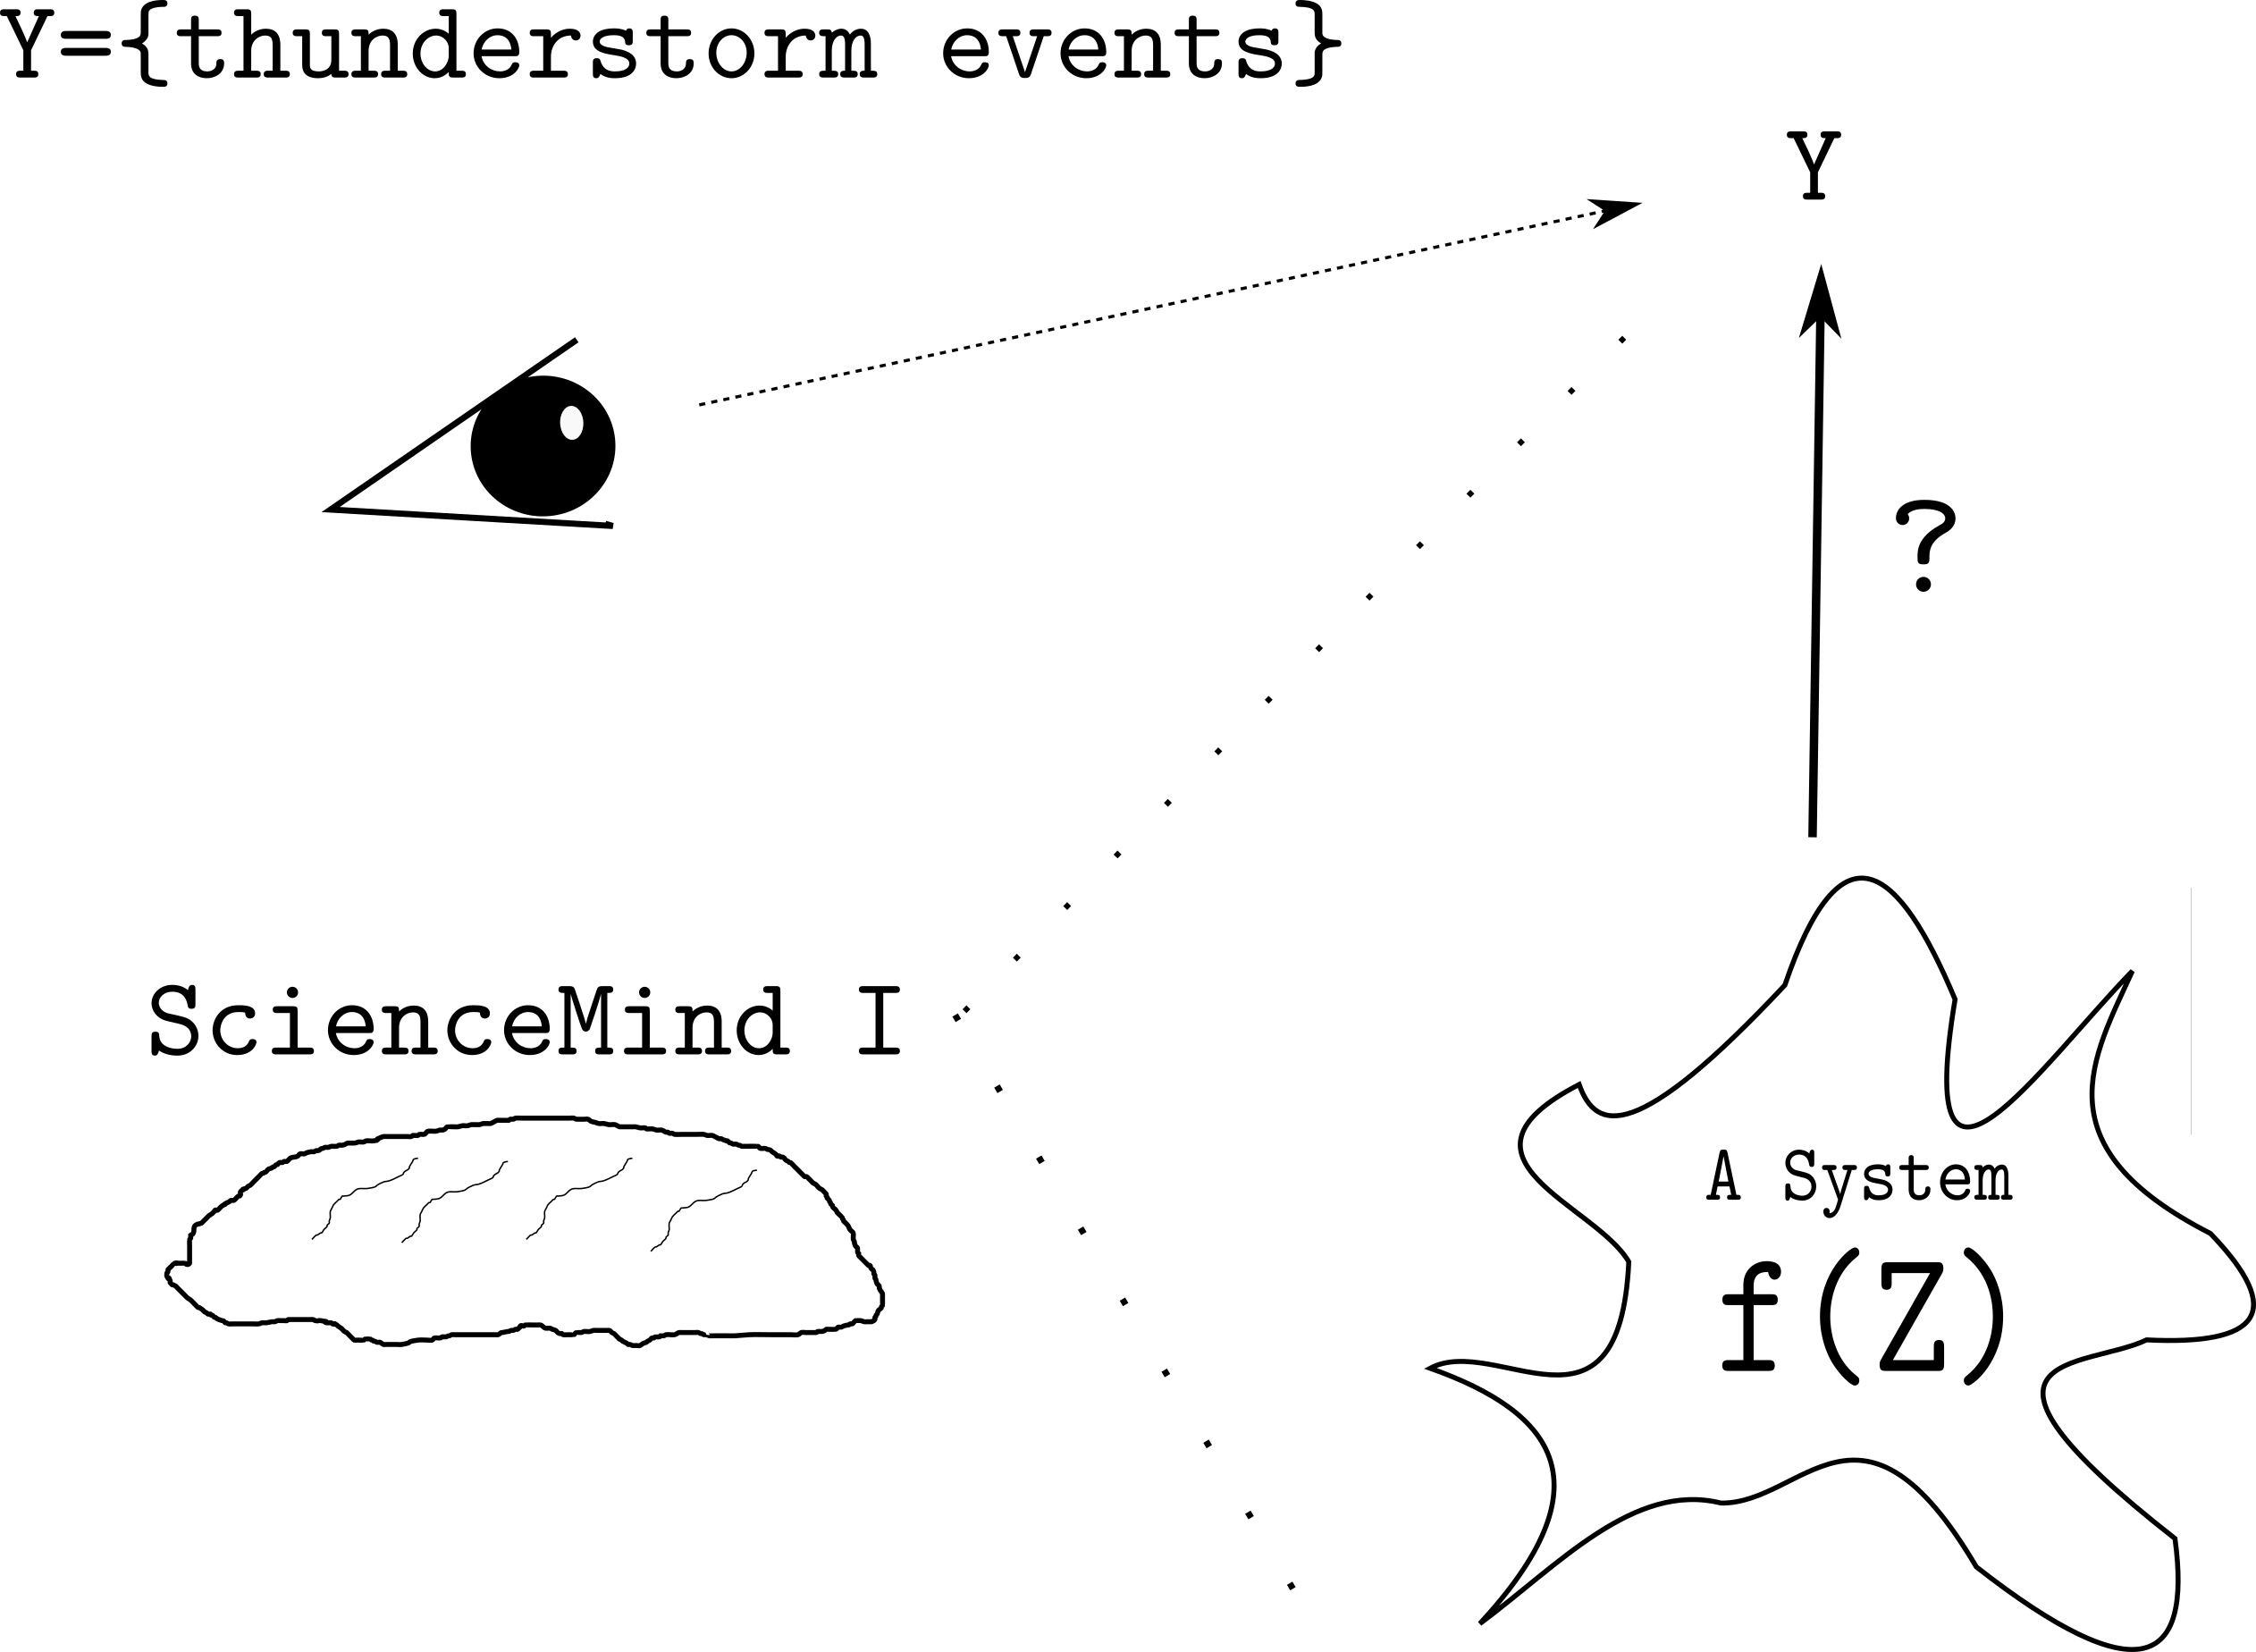
\includegraphics[scale=.75]{graphics/drawing1a}}; 
 \end{tikzpicture}

\end{frame}


%----------------------------------------------------------------
\begin{frame}

\begin{tikzpicture}[overlay]
  \node[anchor=south west] at (1,-4) {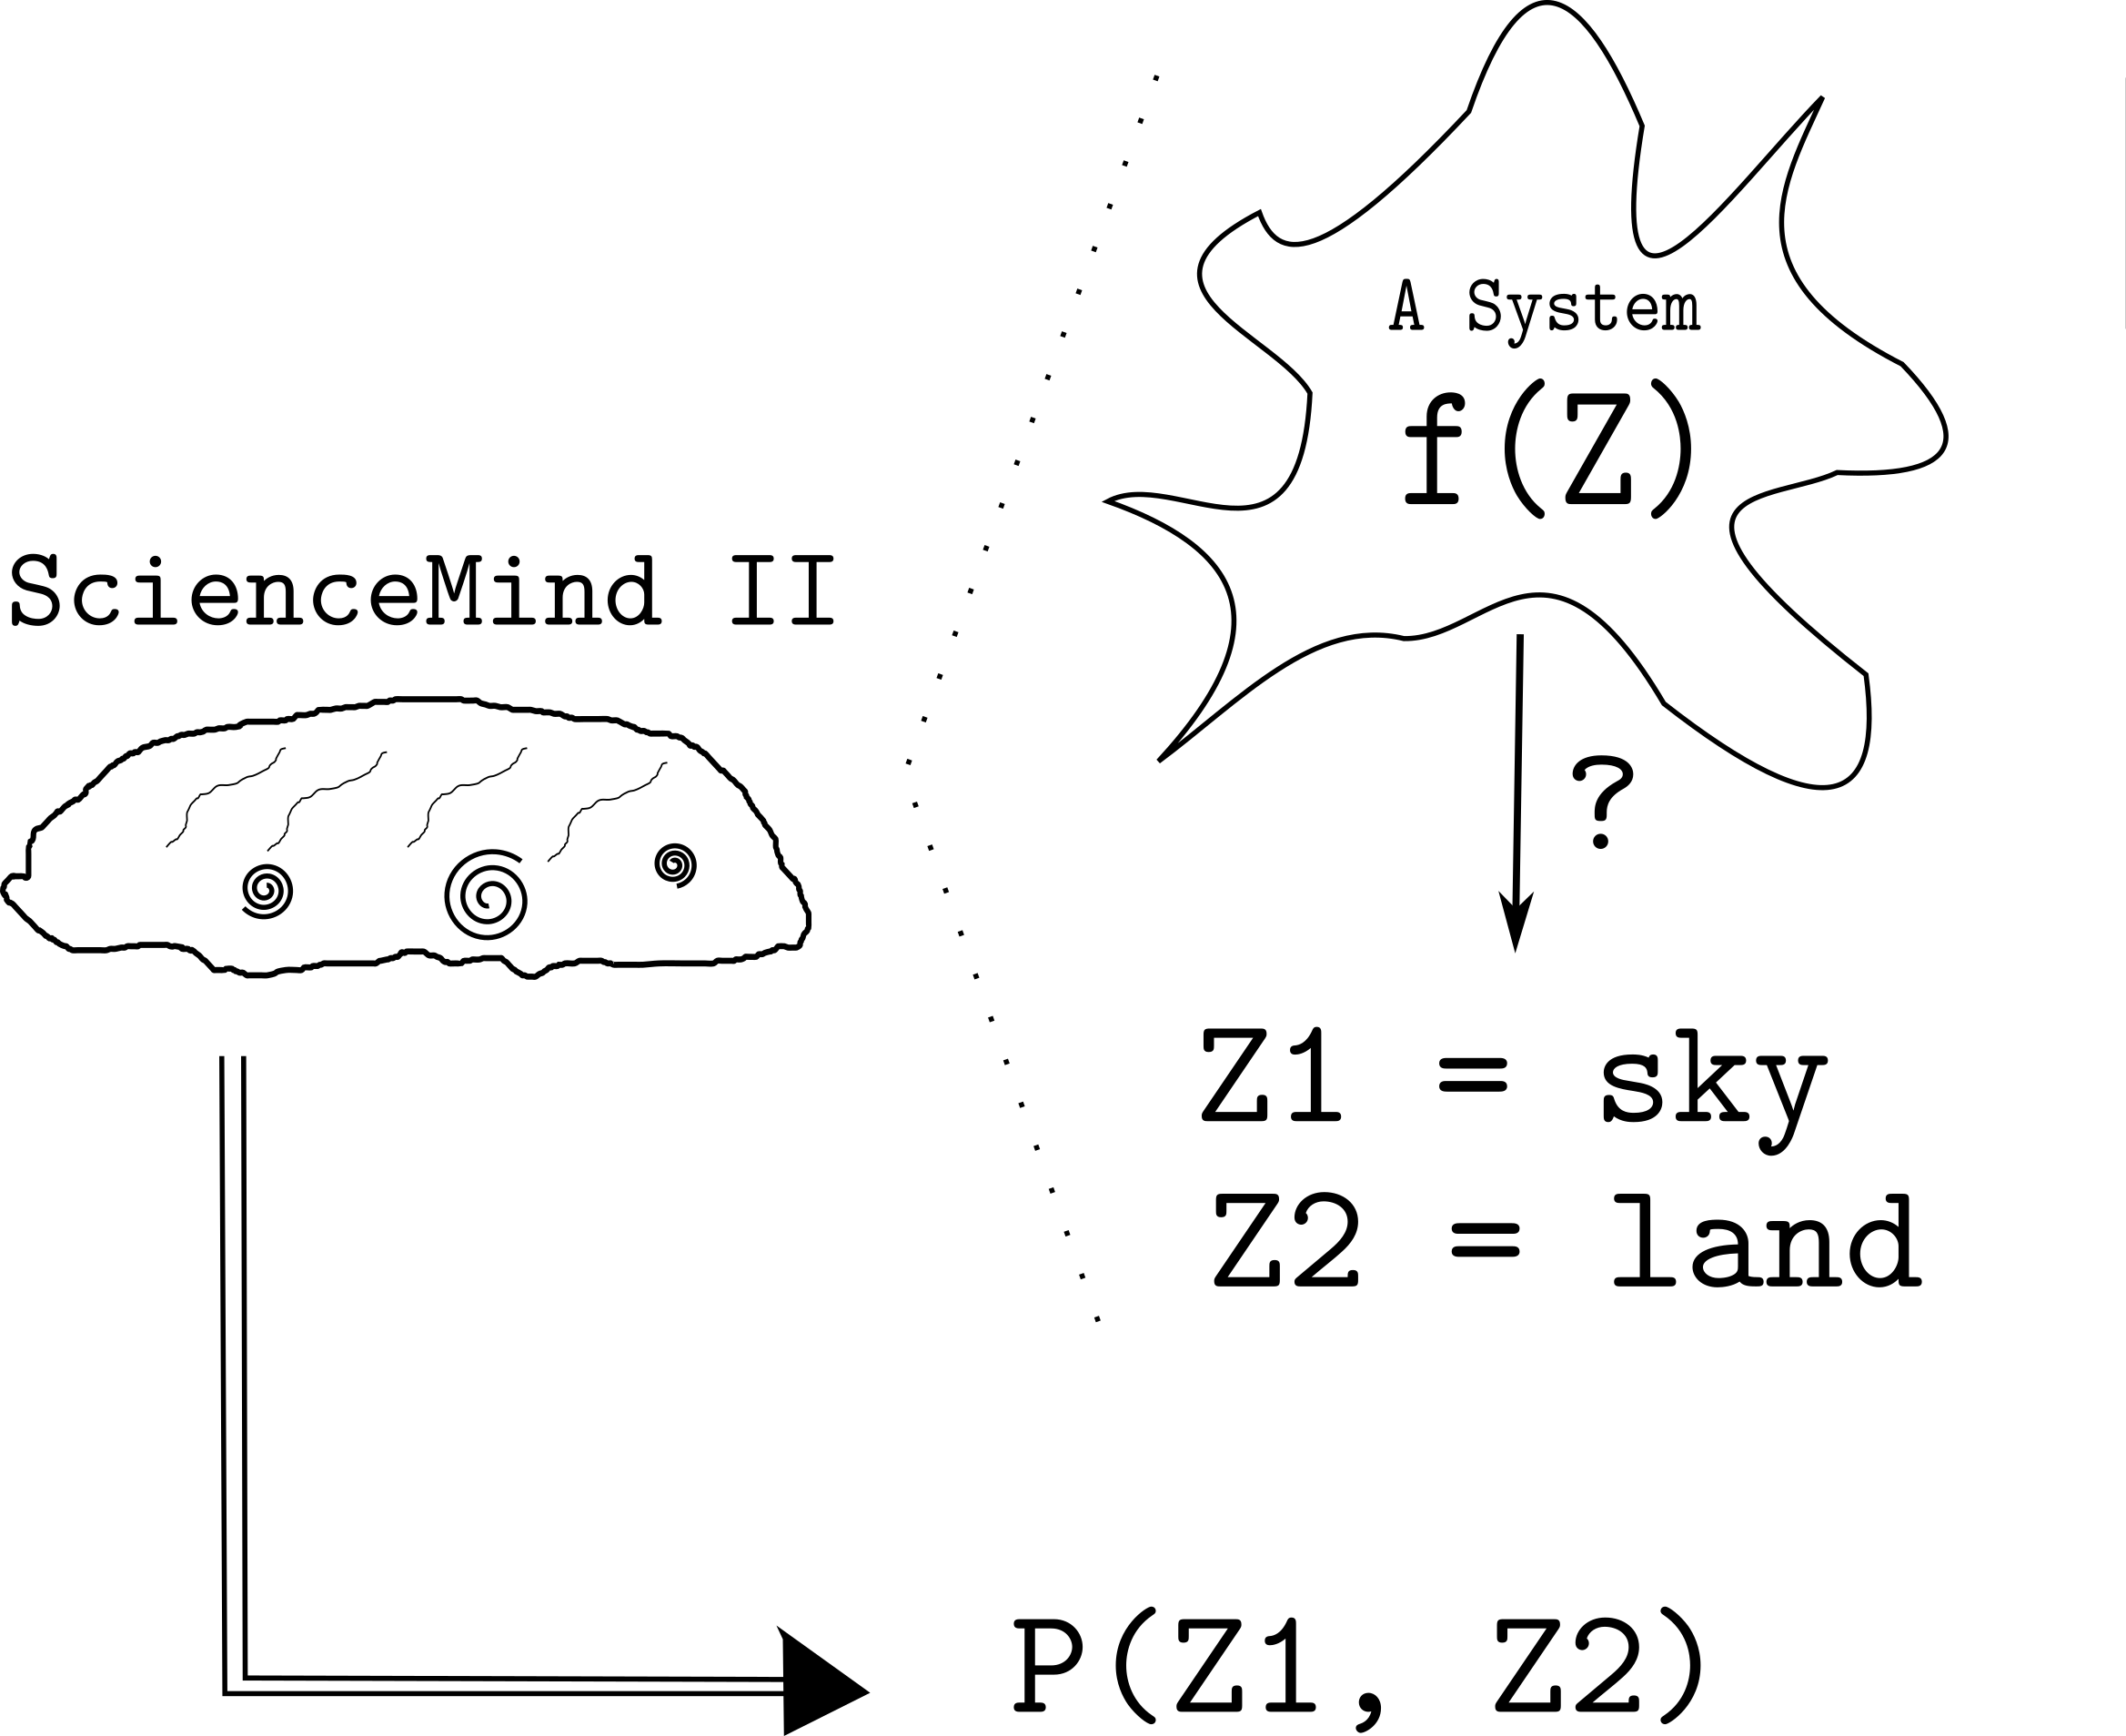
\includegraphics[scale=.70]{graphics/drawing1b}}; 
 \end{tikzpicture}

\end{frame}



%----------------------------------------------------------------
\begin{frame}

\begin{tikzpicture}[overlay]
  \node[anchor=south west] at (1,-4) {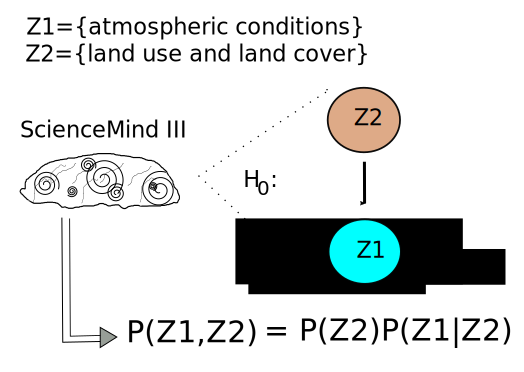
\includegraphics[scale=.70]{graphics/drawing1c}}; 
 \end{tikzpicture}

\end{frame}



%----------------------------------------------------------------
\begin{frame}

\begin{tikzpicture}[overlay]
  \node[anchor=south west] at (0,0.5) {
\includegraphics[scale=.50]{graphics/Ashley1.jpeg}};
  \node[anchor=south west] at (0,-4.0) {
\includegraphics[scale=.50]{graphics/Stallins1.jpeg}};
 \end{tikzpicture}
 
 
 \begin{textblock}{1}(.5,.3)
  \small {... "substantive evidence of urban effects \\ 
  on thunderstorm frequency and severity" ...}
\end{textblock}

 \begin{textblock}{1}(.5,.55)
  \small {"Urban lightning research is still in the \\ 
  descriptive, pattern-identifying stage, \\
  with some inroads into mechanism."}
\end{textblock}

\end{frame}



%----------------------------------------------------------------
\begin{frame}

\begin{tikzpicture}[overlay]
  \node[anchor=south west] at (1.0,-5.5) {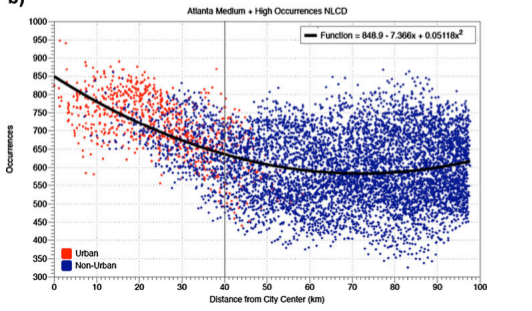
\includegraphics[scale=.75]{graphics/Ashley2.jpeg}}; 
 \end{tikzpicture}
 

\begin{textblock}{1}(.35,.125)
  \footnotesize {$P(Z1, Z2) \ = P(Z2)P(Z1|Z2)$}
\end{textblock}

\begin{textblock}{1}(.15,.155)
  \footnotesize {$(dBZ = decibels \ radar \ reflectivity \Rightarrow  Z1; NLCD \ code \Rightarrow Z2)$}
\end{textblock}


\begin{textblock}{1}(.10,.20)
  \footnotesize{Occurrences $\geq 40$ dBZ for each 2-km grid cell vs. distance from city center}
\end{textblock}
 
 
\begin{textblock}{1}(.75,.72)
  \tiny {Ashley,Bentley,Stallins (2012)}
\end{textblock}

\end{frame}



%----------------------------------------------------------------
\begin{frame}

\begin{tikzpicture}[overlay]
  \node[anchor=south west] at (0,-2.0) {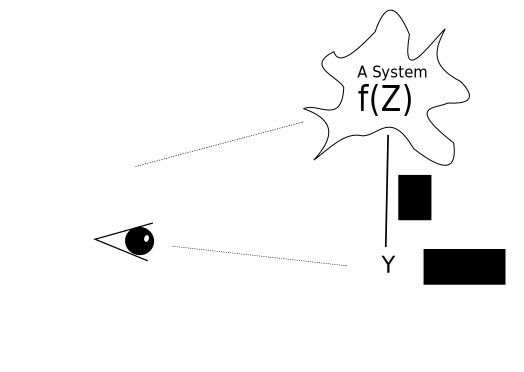
\includegraphics[scale=.35]{graphics/drawing2a}}; 
 \end{tikzpicture}
 
 
 \begin{textblock}{1}(0.40,.25)
  \scriptsize {
  \begin{itemize}
  	\item We observe an entity in Nature that we suspect \\
  	generates non-random patterns of information
  	\item Our states of knowledge about the causal relationships \\
  	and processes, $f(\cdot )$, that are operating as well as about \\
  	the inputs,	$Z$, are limited; often severely	
  	\item We assume that some observable outcome, $Y$, is \\
  	\underline{causally} related to the entity as $f(Z) \Longrightarrow \{Y\}$  	
  \end{itemize}
  }
 \end{textblock}

\end{frame}



%----------------------------------------------------------------
\begin{frame}

\begin{tikzpicture}[overlay]
  \node[anchor=south west] at (0,-2.0) {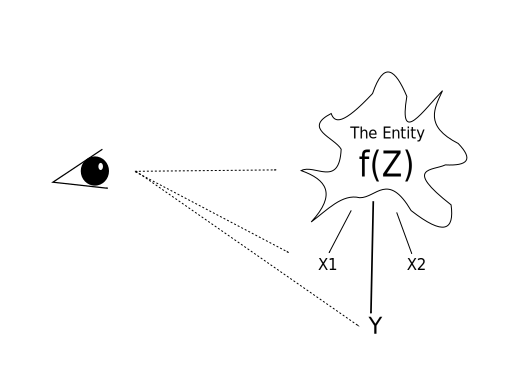
\includegraphics[scale=.35]{graphics/drawing3}}; 
 \end{tikzpicture}
 
 \begin{textblock}{1}(0.40,.25)
  \scriptsize {
  \begin{itemize}
  	\item We assume that some observable and measurable \\
  	attributes (data), $\{X1, X2\}$ are \underline{logically} related \\
  	 to the entity's internal processes as, $\{X1, X2\} | f(Z) $ 
  	\item Lacking full knowledge of the entity's processes, we use \\
  	a probability model and consider $X1, X2, Y$ as random \\
  	variables with a joint probability distribution function
  	\item Lacking complete datasets, we accept sampled datasets
  	\item We make inductive inferences from the sampled datasets \\
  	back to	$f(Z)$ by assuming sampling distributions, \\
  	evaluating our prior knowledge, and using the (weaker) \\
  	syllogisms of plausible reasoning coupled with probability \\
  	theory
  \end{itemize}
  }
 \end{textblock}

\end{frame}



%----------------------------------------------------------------
\begin{frame}



\end{frame}





%######################################
% END DOC
%######################################
\end{document}
